% !TEX program = xelatex
\documentclass[11pt]{article}

\usepackage{fontspec}
\usepackage{unicode-math}
\setmainfont{Latin Modern Roman}
\setsansfont{Latin Modern Sans}
\setmonofont{Latin Modern Mono}[Scale=0.88]

\usepackage{graphicx}
\graphicspath{{figures/}{../../papers/arxiv-ac/figures/}}
\usepackage{booktabs}
\usepackage{tabularx}
\usepackage{ragged2e}
\usepackage{microtype}
\usepackage{natbib}
\usepackage{listings}

\makeatletter
\def\input@path{{../}}
\makeatother
\usepackage{ac-paper-cards}

\hypersetup{
  pdftitle={Playable Folk Songs: Oral Tradition Meets the Browser Keyboard},
}

% Listing style for notepat song notation
\lstdefinestyle{notepat}{
  basicstyle=\ttfamily\small,
  breaklines=true,
  columns=flexible,
  keepspaces=true,
  showstringspaces=false,
}

\begin{document}

% ============================================================
% TITLE CARD
% ============================================================
\thispagestyle{empty}
\vspace*{\fill}
\begin{center}
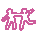
\includegraphics[height=3em]{pals}\par\vspace{0.6em}
{\acbold\fontsize{20pt}{24pt}\selectfont\color{acdark} Playable}\par
{\acbold\fontsize{20pt}{24pt}\selectfont\color{acdark} Folk Songs}\par
\vspace{0.3em}
{\aclight\fontsize{10pt}{12pt}\selectfont\color{acpink} Oral Tradition Meets the Browser Keyboard}\par
\vspace{0.8em}
{\normalsize Jeffrey Alan Scudder}\par
{\small\color{acgray} Aesthetic Inc.}\par
{\small\color{acgray} ORCID: \href{https://orcid.org/0009-0007-4460-4913}{0009-0007-4460-4913}}\par
\vspace{0.3em}
{\small\color{acpurple} \url{https://notepat.com}}\par
\vspace{0.8em}
\rule{0.6\textwidth}{1pt}\par
\vspace{0.4em}
{\small\color{acpink}\textbf{[ working draft --- not for citation ]}}\par
\vspace{0.3em}
{\footnotesize\color{acgray} March 2026}\par
\end{center}
\vspace*{\fill}

% ============================================================
% INDEX CARD
% ============================================================
\cardindex

% ============================================================
% ABSTRACT CARD
% ============================================================
\clearpage
\begin{accentcard}
\cardtitle{Abstract}

Folk songs evolved to be playable without notation, memorizable without instruments, and forkable without permission. These properties---constrained pitch range, repetitive structure, oral transmissibility---make folk melodies structurally ideal for a browser-based keyboard synthesizer.

\vspace{0.3em}

This paper describes the integration of playable folk songs into \np{}.com, a chromatic keyboard instrument that maps QWERTY keys to musical notes. We encode folk melodies in a lightweight \texttt{NOTE:word} format that pairs each pitch with its lyric syllable, creating a guided performance mode where the instrument teaches the song one note at a time.

\vspace{0.3em}

We survey folk melody collections suitable for this encoding, analyze why folk songs' structural constraints align with keyboard-as-instrument interfaces, and argue that the folk process---variation, selection, oral transmission---has a natural digital analogue in URL-shareable, forkable song encodings.
\end{accentcard}

% ============================================================
% SECTION 1: THE ARGUMENT
% ============================================================
\section{The Argument}

Folk songs are humanity's oldest open-source software.

They have no single author. They are maintained by a community. They are transmitted orally---meaning they must be simple enough to memorize, constrained enough to reproduce, and flexible enough to adapt. Every singer is a contributor; every performance is a fork.

\vspace{0.3em}

These are exactly the properties that make a melody playable on a QWERTY keyboard.

\begin{card}
\cardtitle{Why Folk Songs?}
\begin{itemize}
  \item \textbf{Narrow pitch range}: Most folk melodies span 1--1.5 octaves~\citep{lomax1968folk}. \np{}'s two-octave button grid covers them entirely.
  \item \textbf{Pentatonic bias}: Many traditions favor 5-note scales~\citep{kodaly1971folk}, reducing the cognitive load of finding the next note.
  \item \textbf{Repetitive structure}: 8-bar phrases that repeat, call-and-response patterns, verse--chorus forms---all aid memorization and guided playback.
  \item \textbf{No wrong notes}: In pentatonic melodies, adjacent scale tones are consonant. The Orff Schulwerk method exploits this same property with removable xylophone bars~\citep{orff1978schulwerk}.
\end{itemize}
\end{card}

% ============================================================
% SECTION 2: THE INSTRUMENT
% ============================================================
\section{The Instrument}

\np{}.com is a browser-based chromatic synthesizer built as a ``piece'' (interactive program) inside \ac{}~\citep{scudder2026ac, scudder2026notepat}. It maps the QWERTY keyboard to 24 chromatic notes across two octaves, with octave shifting to cover the full piano range.

\begin{darkcard}
\textbf{Song mode} transforms \np{} from a free-play instrument into a guided performance interface. A scrolling lyric track shows the current syllable; only the correct note is active; pressing it advances to the next syllable. The player cannot make a mistake---they can only wait.
\end{darkcard}

This ``training wheels'' approach---blocking wrong notes, highlighting the right one---mirrors the Orff and Kod\'aly pedagogies, which constrain the instrument to match the learner's current ability~\citep{kodaly1971folk, orff1978schulwerk}.

% ============================================================
% SECTION 3: THE ENCODING
% ============================================================
\section{The Encoding}

Songs in \np{} are encoded as whitespace-separated \texttt{NOTE:word} pairs:

\notesong{C:Twin- C:-kle G:twin- G:-kle A:lit- A:-tle G:star,\\
F:how F:I E:won- E:-der D:what D:you C:are.}

Each token is a note name (\texttt{C}, \texttt{G}, \texttt{A}, \texttt{F\#}, etc.) paired with a lyric syllable via colon. Hyphens indicate syllable continuation: a trailing hyphen (\texttt{Twin-}) means the next token continues the same word; a leading hyphen (\texttt{-kle}) is the continuation.

\begin{card}
\cardtitle{Design Properties}
\begin{itemize}
  \item \textbf{Human-readable}: A musician can sight-read the encoding directly.
  \item \textbf{URL-safe}: Songs can be passed as URL parameters to \np{}.
  \item \textbf{Forkable}: Copy, edit, share---the folk process in a text string.
  \item \textbf{Minimal}: No duration, no dynamics, no tempo. The player controls all three.
\end{itemize}
\end{card}

The absence of rhythm information is deliberate. In oral tradition, rhythm belongs to the performer, not the score~\citep{lomax1968folk}. The encoding captures \emph{what} to play; the player decides \emph{how}.

% ============================================================
% SECTION 4: A CATALOG
% ============================================================
\section{A Catalog of Playable Melodies}

We surveyed folk song collections from multiple traditions and selected melodies optimized for \np{}'s two-octave grid. Selection criteria: pitch range $\leq$\,15 semitones, pentatonic or simple diatonic scale, and cultural recognizability.

\begin{card}
\cardtitle{Pentatonic (5 notes)}
\begin{tabularx}{\linewidth}{Xll}
\toprule
\textbf{Song} & \textbf{Origin} & \textbf{Range} \\
\midrule
Amazing Grace & American & P5+oct \\
Auld Lang Syne & Scottish & oct \\
Arirang & Korean & oct \\
Sakura & Japanese & m7 \\
Mo Li Hua & Chinese & oct \\
Swing Low & Spiritual & oct \\
\bottomrule
\end{tabularx}
\end{card}

\begin{card}
\cardtitle{Narrow Range ($<$ octave)}
\begin{tabularx}{\linewidth}{Xll}
\toprule
\textbf{Song} & \textbf{Origin} & \textbf{Range} \\
\midrule
Mary Had a Little Lamb & American & P5 \\
Hot Cross Buns & English & M3 \\
Fr\`ere Jacques & French & M6 \\
London Bridge & English & P5 \\
Korobeiniki & Russian & oct \\
\bottomrule
\end{tabularx}
\end{card}

\begin{card}
\cardtitle{Modal \& Diatonic}
\begin{tabularx}{\linewidth}{Xll}
\toprule
\textbf{Song} & \textbf{Origin} & \textbf{Range} \\
\midrule
Greensleeves & English & 10th \\
Scarborough Fair & English & oct \\
Danny Boy & Irish & 10th \\
Shenandoah & American & 10th \\
Hava Nagila & Israeli & oct \\
\bottomrule
\end{tabularx}
\end{card}

% ============================================================
% SECTION 5: FOLK PROCESS AS VERSION CONTROL
% ============================================================
\section{The Folk Process as Version Control}

The International Folk Music Council identified three properties of the folk process: \emph{continuity} (linking present to past), \emph{variation} (creative impulse of individual performers), and \emph{selection} (community determines which forms survive)~\citep{karpeles1955definition}.

\begin{accentcard}
These map directly onto software version control:

\vspace{0.3em}
\begin{tabularx}{\linewidth}{lX}
\textbf{Continuity} & \texttt{main} branch \\
\textbf{Variation} & commits, forks \\
\textbf{Selection} & merge decisions, adoption \\
\end{tabularx}
\end{accentcard}

A \np{} song encoding is a URL. Sharing a song is sharing a link. Modifying a song is editing a text string and sharing a new link. The ``oral tradition'' becomes a tradition of URLs---the melody transmits not through memory but through hypertext.

This is not metaphorical. The Essen Associative Code (ESAC) database, started in 1982, encoded $\sim$8,000 European and Chinese folk songs in a computer-friendly notation inspired by Chinese \textit{jianpu}~\citep{schaffrath1995esac}. \np{}'s \texttt{NOTE:word} format is a direct descendant of this tradition: encoding melody as text so that computation and transmission become possible.

% ============================================================
% SECTION 6: COMPUTATIONAL MUSICOLOGY
% ============================================================
\section{Computational Dimensions}

Passmore et al.\ modeled folk melodies as evolving sequences from a 12-pitch ``alphabet,'' applying sequence alignment methods borrowed from molecular genetics to 10,062 Japanese and English melodies~\citep{passmore2023cultural}. They found that note changes with smaller melodic impact are more likely to survive---a selection pressure that favors the simplicity folk songs are known for.

\begin{card}
\cardtitle{Why This Matters for \np{}}

If folk melodies are subject to evolutionary selection pressure toward simplicity, then they are \emph{converging} on the properties that make them playable on constrained interfaces. The QWERTY keyboard is not an impoverished substitute for a piano---it is a constraint that matches the constraint the folk process already applies.
\end{card}

Lomax's cantometrics project coded 37 aspects of performance style across 5,776 songs from 1,026 societies, finding that performance style (not melodic content) was the primary cultural indicator~\citep{lomax1968folk}. This supports \np{}'s design decision to encode pitch but not rhythm: the culturally significant variation happens in \emph{how} the notes are performed, which is exactly what the player controls.

% ============================================================
% SECTION 7: RELATED INSTRUMENTS
% ============================================================
\section{Related Instruments}

\begin{card}
\cardtitle{aQWERTYon}
NYU's Music Experience Design Lab built the aQWERTYon, a browser instrument mapping QWERTY keys to scale degrees so there are ``no wrong notes''~\citep{hein2017aqwertyon}. \np{} differs in two ways: it uses \emph{chromatic} mapping (wrong notes are possible and pedagogically useful), and it pairs notes with lyrics (the song teaches itself).
\end{card}

\begin{card}
\cardtitle{ABC Notation}
The de facto standard for folk music encoding, ABC notation represents melody as text~\citep{walshaw2011abc}. The \texttt{abcjs} library renders ABC as interactive sheet music in browsers. \np{}'s encoding is simpler---no duration, no barlines---because it is not a notation system but a \emph{performance script}: it tells the player what to press, not what the music looks like.
\end{card}

\begin{card}
\cardtitle{Tunepal}
A music information retrieval system connecting musicians to 13,290 traditional Irish tunes via query-by-playing~\citep{duggan2009tunepal}. Tunepal finds tunes; \np{} teaches them. They are complementary.
\end{card}

% ============================================================
% SECTION 8: THE BARE-METAL FOLK INSTRUMENT
% ============================================================
\section{The Bare-Metal Folk Instrument}

\np{} runs not only in browsers but on bare metal---a 987-line QuickJS port that boots as PID~1 on AC Native OS~\citep{scudder2026os}. A laptop running \np{} on bare metal is, in a literal sense, a folk instrument: a single-purpose device for playing songs, with no operating system, no desktop, no distractions.

\begin{accentcard}
The convergence is complete: folk songs, designed to be played on the simplest available instrument, running on the simplest possible computer---a Linux kernel, a framebuffer, and a keyboard.
\end{accentcard}

% ============================================================
% SECTION 9: FUTURE WORK
% ============================================================
\section{Future Work}

\begin{card}
\begin{itemize}
  \item \textbf{Crowdsourced encoding}: A public repository of \texttt{NOTE:word} encodings, submitted as URLs, versioned like folk songs themselves.
  \item \textbf{Cross-cultural collections}: Encoding melodies from the Essen, Roud, and Lomax archives into \np{} format, with permission and attribution.
  \item \textbf{Adaptive difficulty}: Expanding pitch range as the player masters simpler songs---a Kod\'aly-like progression through the folk repertoire.
  \item \textbf{Multiplayer folk sessions}: Two \np{} players on the same song, one playing melody, one playing harmony---a digital \textit{session} in the Irish traditional sense.
  \item \textbf{Recording and sharing}: Capture a performance as audio, pair it with the encoding URL, and post it---an oral tradition with receipts.
\end{itemize}
\end{card}

% ============================================================
% CONCLUSION CARD
% ============================================================
\section{Conclusion}

Folk songs survived centuries without notation, without recording, without instruments. They survived because they were simple enough to remember, flexible enough to adapt, and valuable enough to share.

A browser keyboard that teaches these songs one note at a time is not a departure from the folk tradition. It \emph{is} the folk tradition---adapted, once more, to the instrument at hand.

\vspace{0.5em}
\noindent\textbf{ORCID:} \href{https://orcid.org/0009-0007-4460-4913}{0009-0007-4460-4913}

\bibliographystyle{plainnat}
\bibliography{references}

\end{document}
